% include the figures path relative to the master file
\graphicspath{ {./content/method/figures/} }

\section{Data}\label{sec:data}
A common dataset is required to compare different methodologies.
Despite the fact that lack of public data is a common claim in the medical image community~\cite{giger2008anniversary}, the ophtalmic community has recently made available public dataset, mainly gathered at Duke University~\cite{farsiu2014quantitative,Srinivasan2014}.
Although these datasets have been used by Venhuizen~\emph{et~al.}~\cite{Venhuizen2015} and Srinivasan~\emph{et~al.}~\cite{Srinivasan2014}, they are not suitable for our problem.

Venhuizen~\emph{et~al.} have evaluated their framework on a large public dataset of $384$ \gls{oct} annotated volumes classified either as \gls{amd} or normal cases.
Our goal, however, remains to focus on the detection of \gls{dme} rather than \gls{amd}, despite the interest of testing the frameworks against a large dataset.

In the contrary, Srinivasan~\emph{et~al.} have tested their framework using a public dataset containing \gls{amd}, \gls{dme}, and normal volumes~\cite{Srinivasan2014}.
The data, however, have been denoised, aligned, and cropped, without access to the original set of images.

Therefore, we use the \gls{seri} dataset to conduct this study~\cite{seri2016apr-repoICPR}.
This dataset has been acquired by the \gls{seri}, using CIRRUS TM (Carl Zeiss Meditec, Inc., Dublin, CA) \gls{sdoct} device.
The dataset consists of 32 \gls{oct} volumes, subdivided into 16 \gls{dme} and 16 normal cases.
Each volume contains $128$ B-scans with a resolution of \SI[product-units=repeat]{512x1024}{\px}.
All \gls{sdoct} images have been read and assessed by trained graders and identified as normal or \gls{dme} cases, based on evaluation of retinal thickening, hard exudates, intraretinal cystoid space formation and subretinal fluid (see Fig.\,\ref{fig:bbdd}).

\begin{figure*}
\begin{center}
   \subfigure[Vitreomacular traction.]{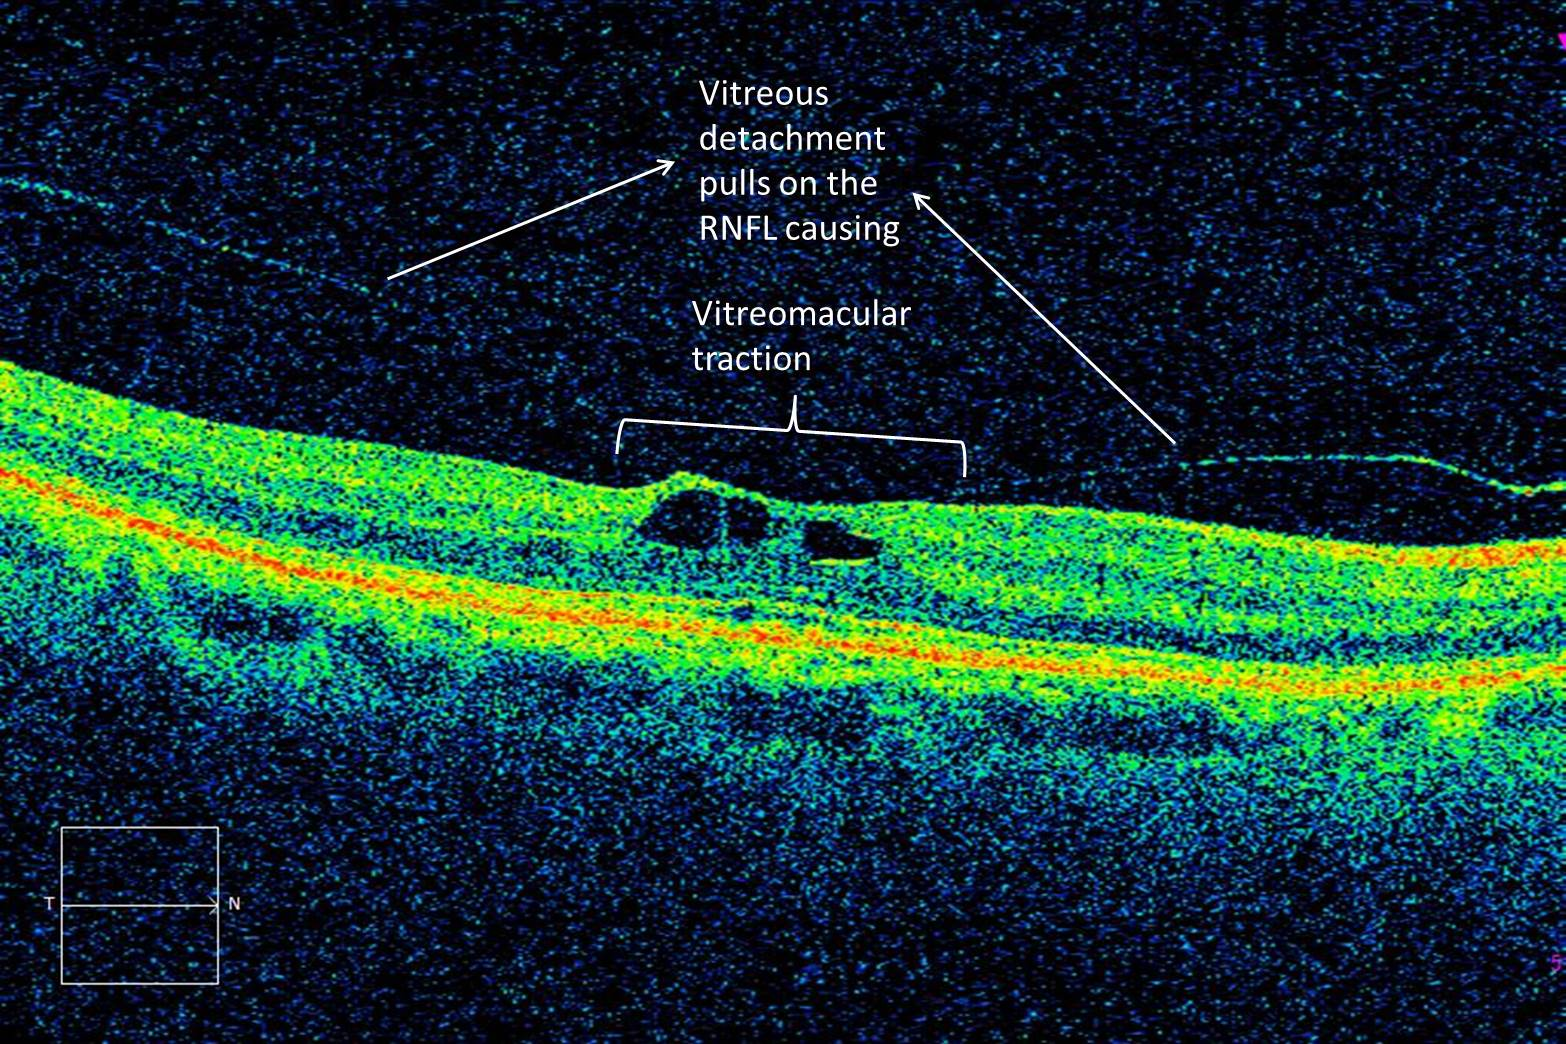
\includegraphics[width=0.3\textwidth, height = 0.15\textheight]{Vitreomacular}}\
   \subfigure[Rethinal thickening.]{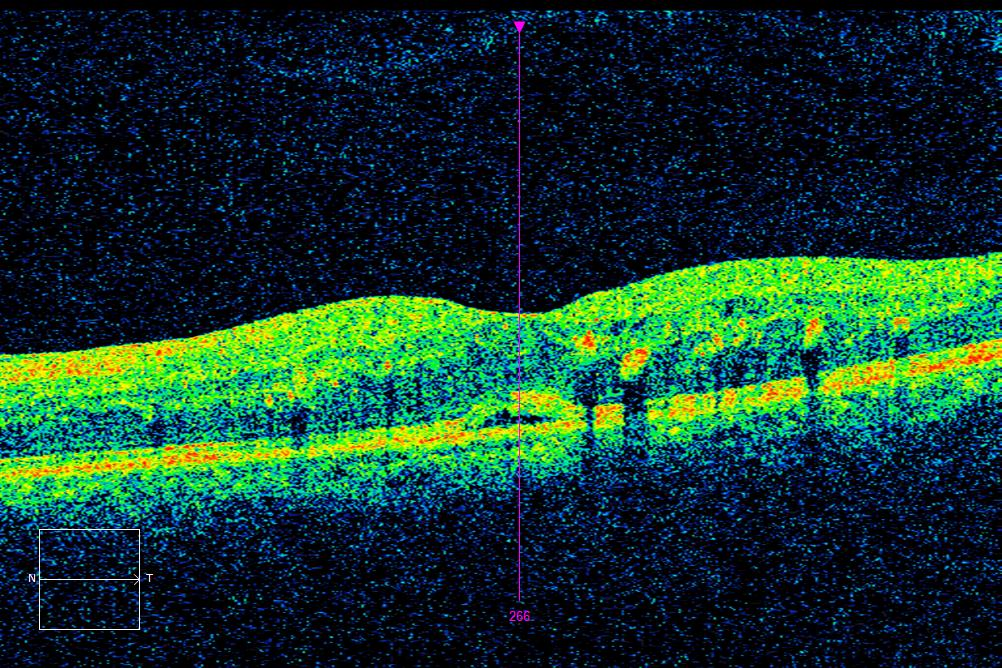
\includegraphics[width = 0.3\textwidth,height = 0.15\textheight]{RE}} \
   \subfigure[Cyst spaces, causing central and parafoveal retina thickening.]{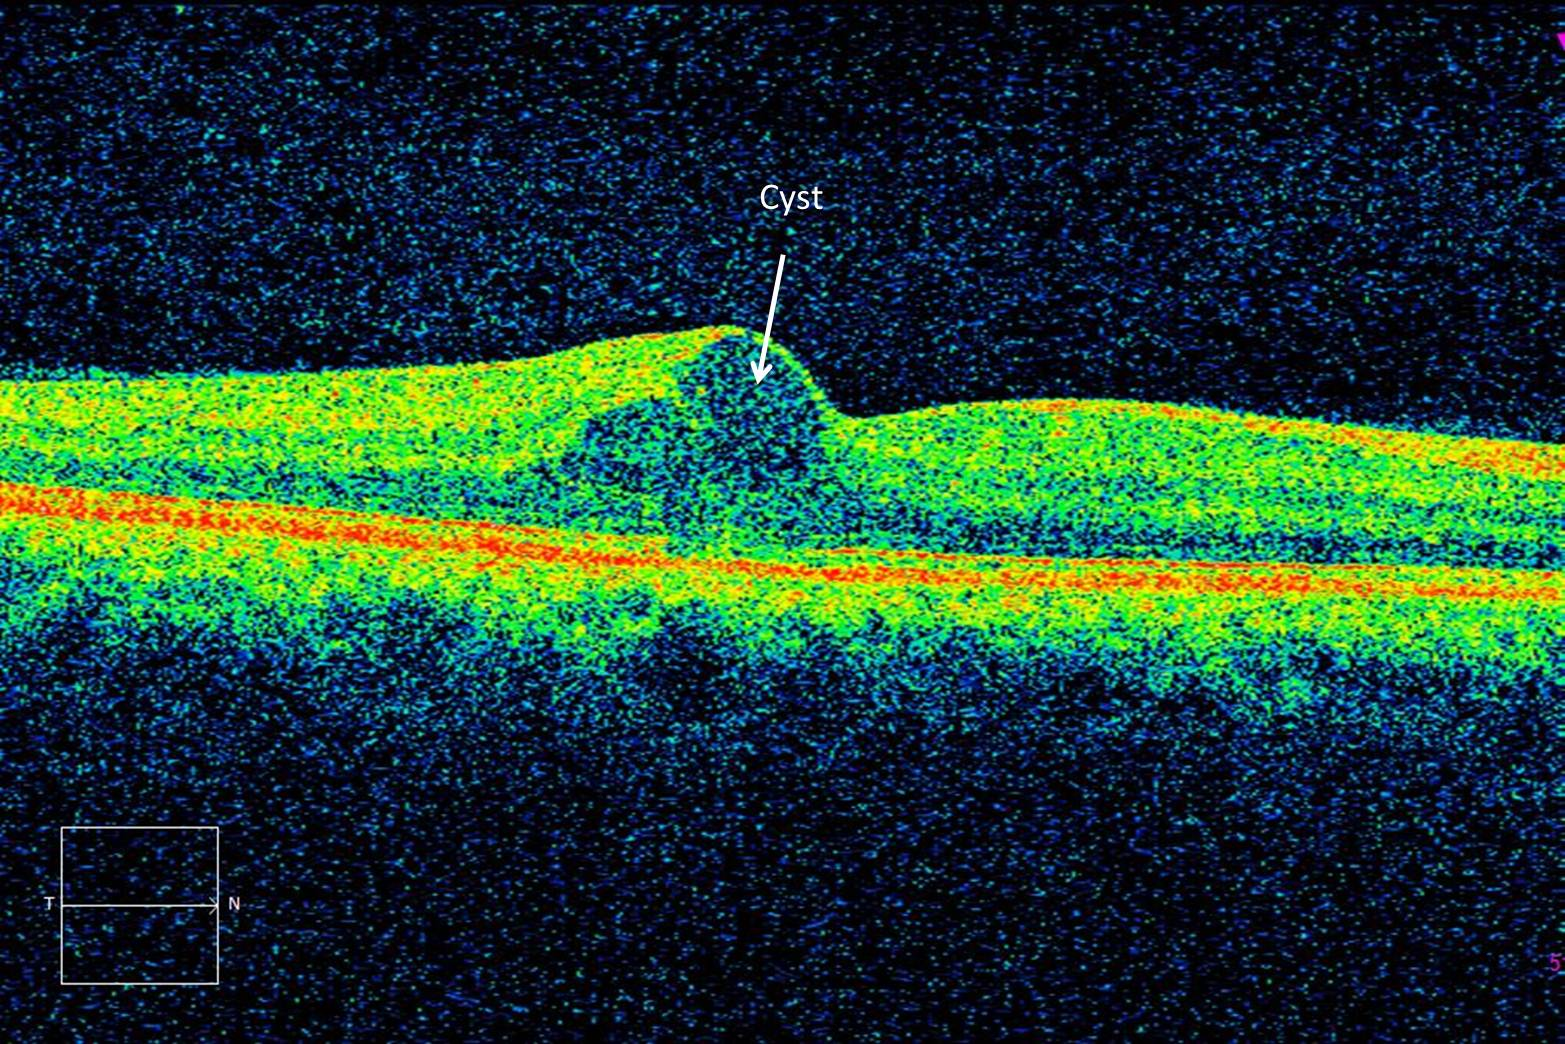
\includegraphics[width=0.3\textwidth,height = 0.15\textheight]{Cyst}}\\
   \subfigure[Cyst spaces and hard exudates, causing central retinal thickening.]{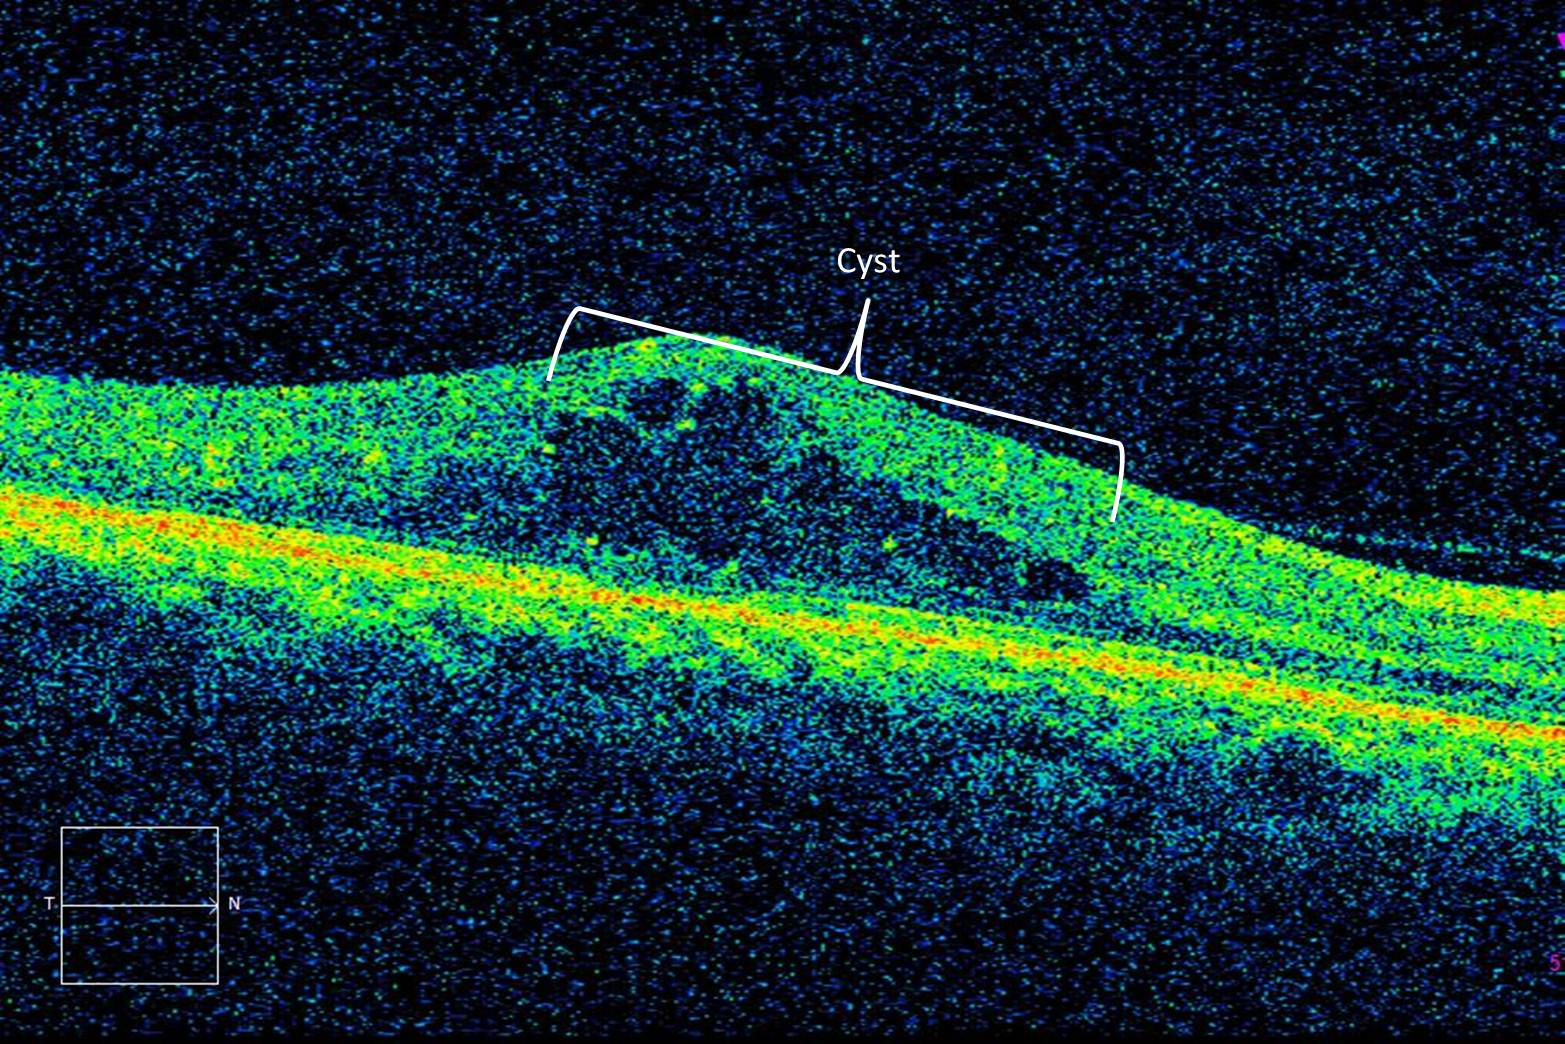
\includegraphics[width = 0.3\textwidth,height = 0.15\textheight]{Cyst+HE+RE}} \
   \subfigure[CSR (subretinal fluid), causing central and parafoveal thickening.]{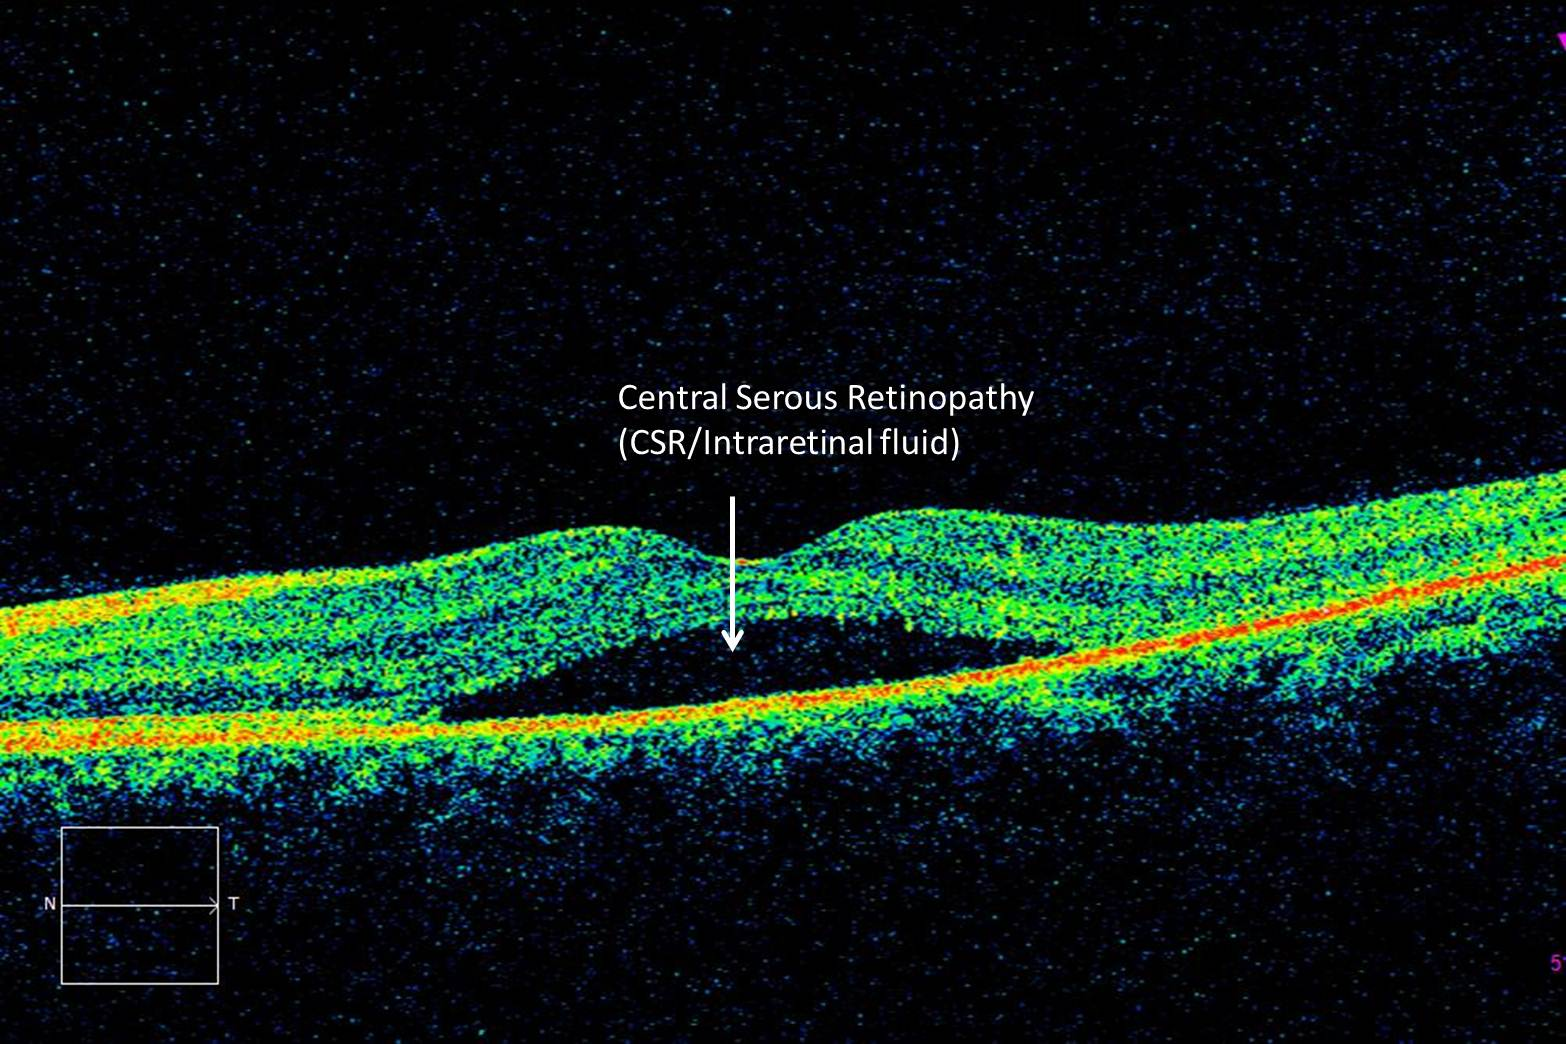
\includegraphics[width = 0.3\textwidth,height = 0.15\textheight]{CSR}} \
   \subfigure[CSR, hard exudates and cyst spaces.]{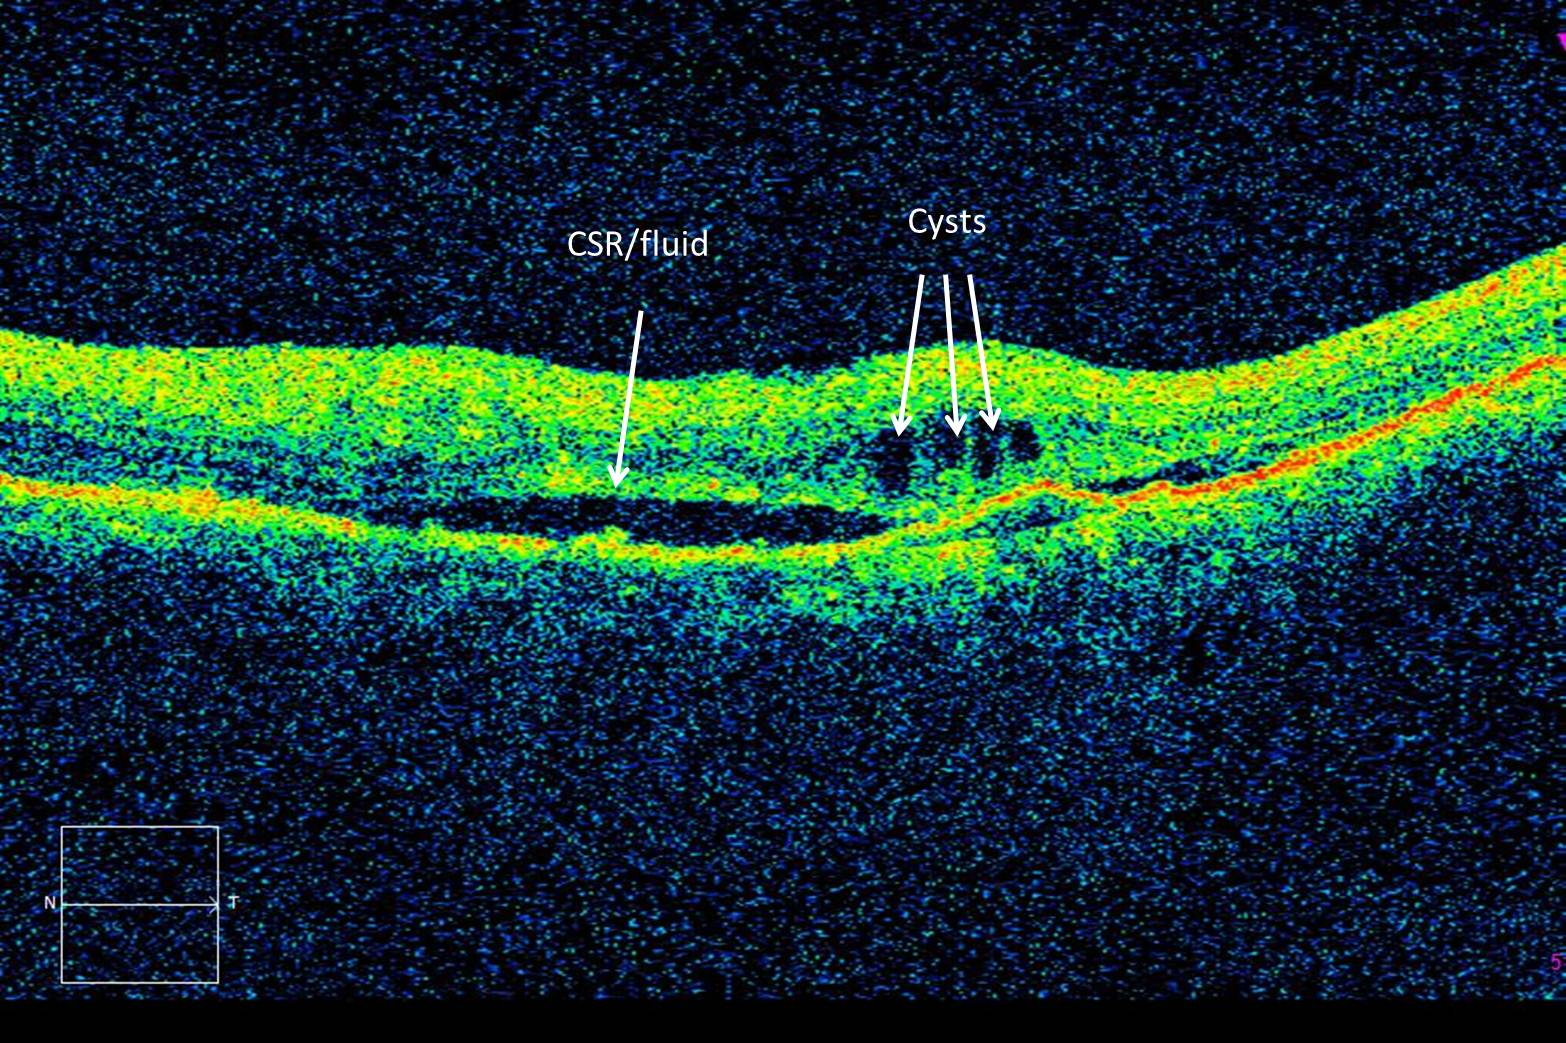
\includegraphics[width = 0.3\textwidth,height = 0.15\textheight]{Cyst+CSR+HE}} \\
   \subfigure[Cyst spaces, causing retinal thickening.]{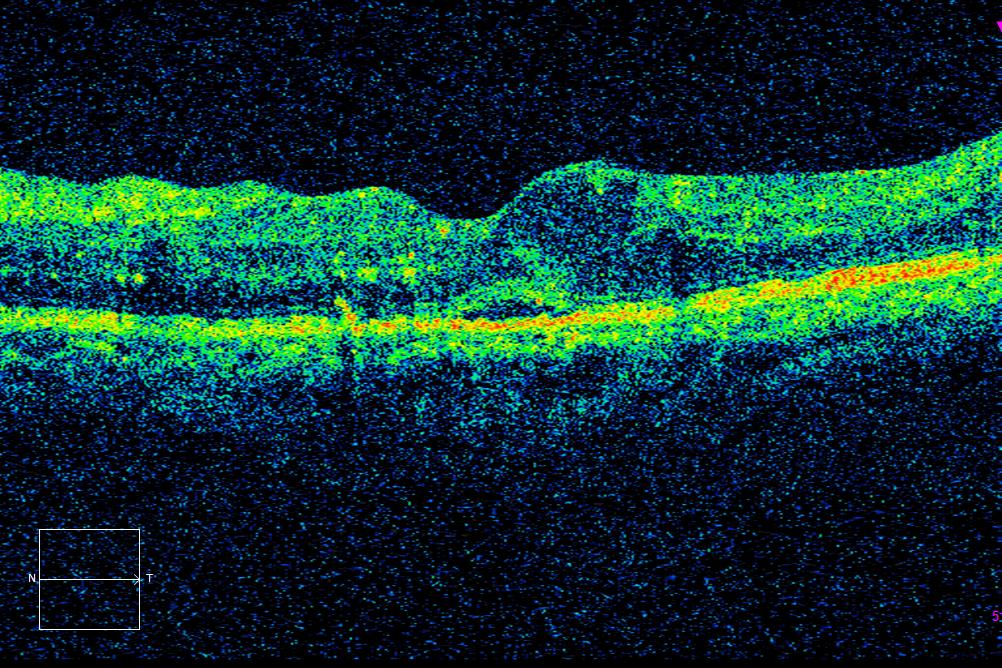
\includegraphics[width = 0.3\textwidth,height = 0.15\textheight]{Cyst+RE}} \
   \subfigure[CSR and hard exudates, causing retinal thickening.]{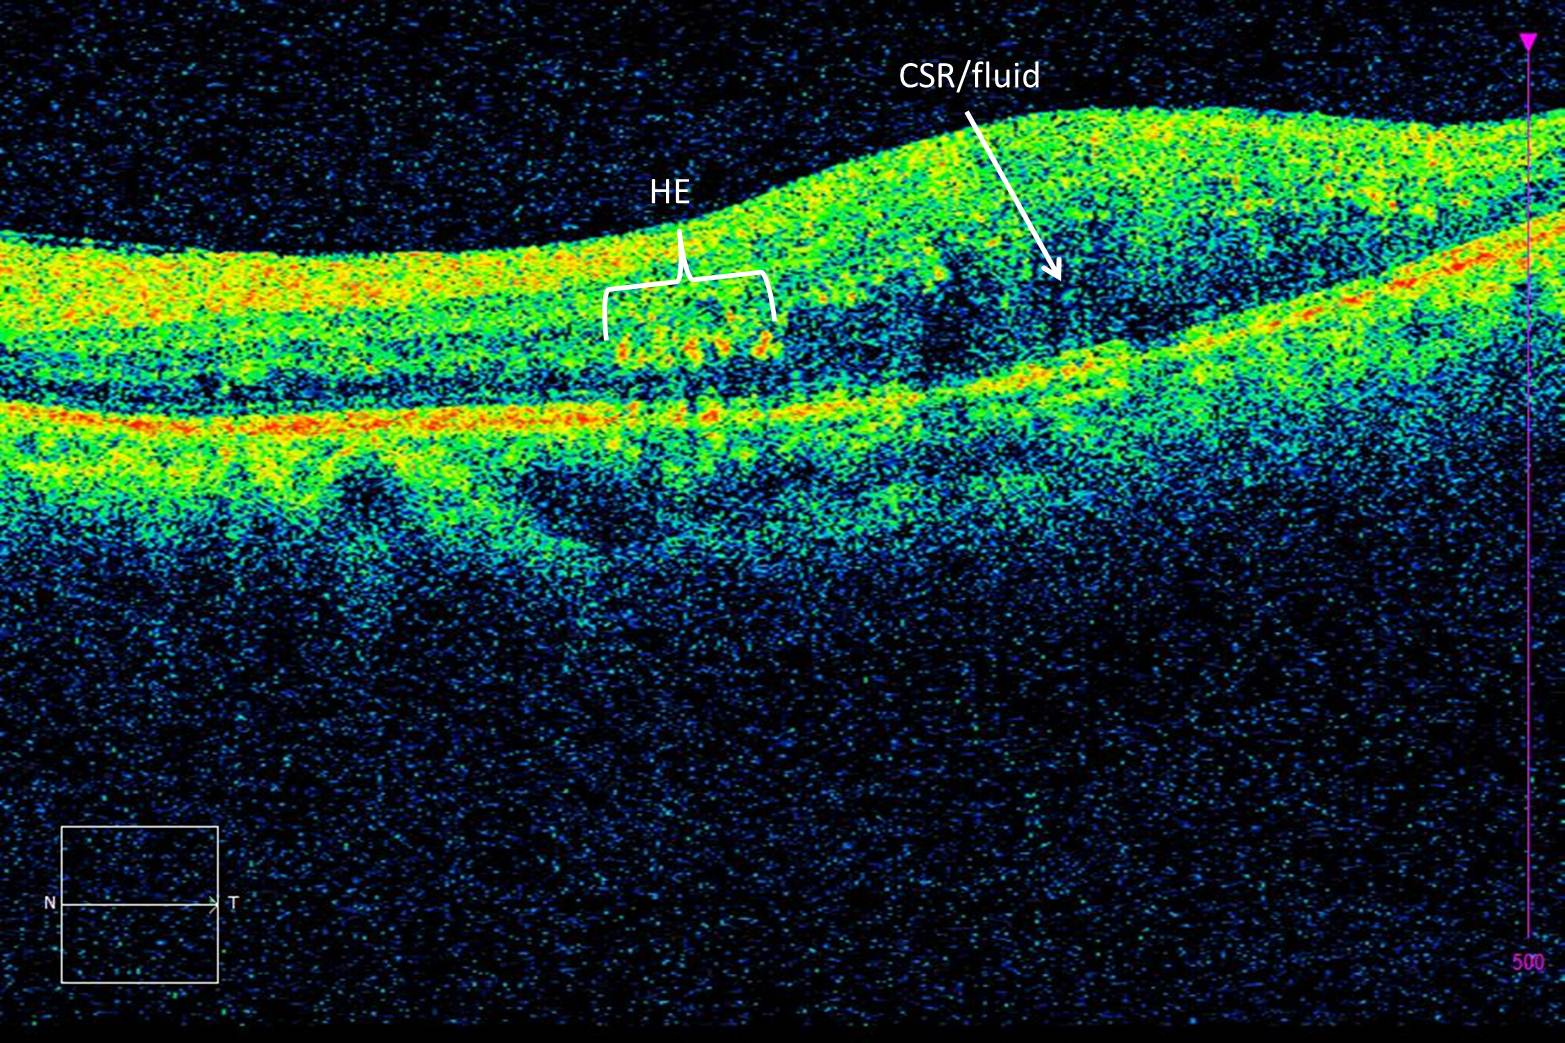
\includegraphics[width = 0.3\textwidth,height = 0.15\textheight]{CSR+HE+RE}} \   
   \subfigure[Cyst spaces causing parafoveal thickening.]{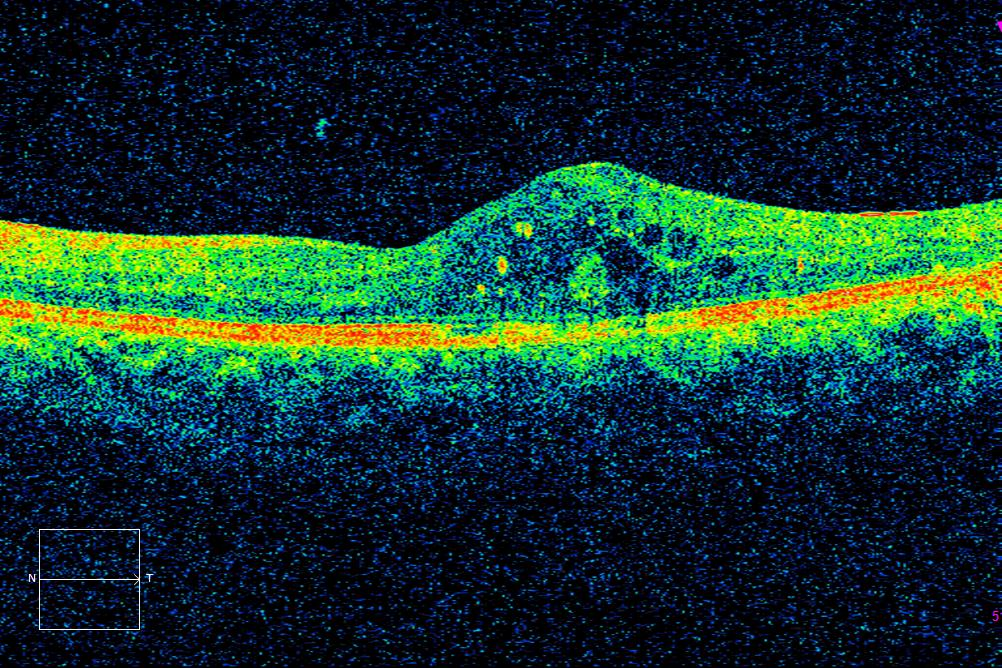
\includegraphics[width = 0.3\textwidth,height = 0.15\textheight]{Cyst+RE_parafovel}} \\
    
\end{center}
    \caption{Examples of \gls{dme} cases in \gls{seri} dataset.}
  \label{fig:bbdd}
\end{figure*}
% 4, 2, 1\\
% 1, 1, 1\\
% 3, 2, 1\\
